\documentclass{beamer}

\usetheme{Warsaw}
 %\usetheme{Ilmenau}
\usepackage[style=verbose]{biblatex}
\bibliography{bib}
%\usetheme{CambridgeUS}

%\usetheme{Singapore}


\usefonttheme{serif}


\expandafter\def\expandafter\insertshorttitle\expandafter{%
	\insertshorttitle\hfill%
	\inserttotalframenumber\,/\,\insertframenumber}

\usepackage{ptext}
\usepackage{xepersian}
\settextfont[Scale=1]{Yas}
\usefonttheme{professionalfonts}
\definecolor{studentbrown}{RGB}{124,71,50}
\include{tashih}
\include{commands}

\begin{document}

\title{جداسازی کور مخلوط‌های غیرخطی فرآیند‌های تصادفی}
\subtitle{ارائه‌ی نهایی پروژه‌ی کارشناسی یک}
\author[بهراد منیری]{
	بهراد منیری\\
	\footnotesize\url{bemoniri@ee.sharif.edu} \\\vspace{0.9cm}
	استاد راهنما:\\
	دکتر مسعود بابائی‌زاده}

\institute[دانشگاه‌ صنعتی شریف]{
	دانشکده‌ی مهندسی برق\\
	دانشگاه صنعتی شریف
}

\date{}

\begin{frame}
\maketitle
\end{frame}

%\begin{frame}
%\tableofcontents
%\end{frame}

\begin{frame}{جداسازی کور منابع}
\frametitle{جداسازی کور منابع: معرفی مسئله}

\begin{figure}
	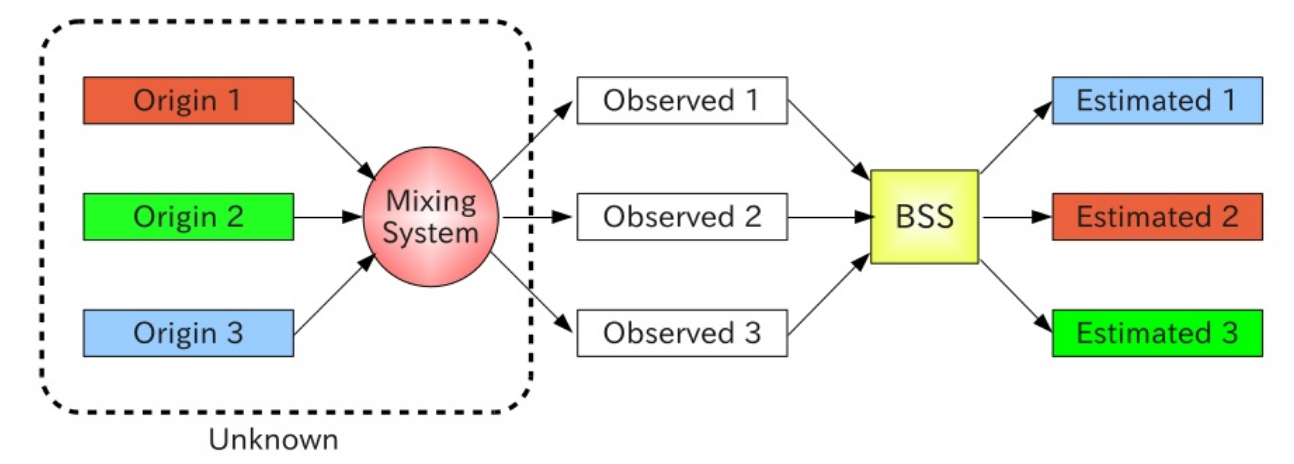
\includegraphics[scale=0.25]{slide1.png}
\end{figure}
\end{frame}

%\begin{frame}
%\frametitle{انگیزه‌ی حل مسئله}
%\begin{itemize}
%	\item 
%	جداسازی صوت (مسئله‌ی مهمانی)
%	
%	\item
%	جداسازی در تصاویر
%	
%	\item
%	جداسازی منابع در سیگنال‌های الکتروانسفالوگرام
%\end{itemize}
%
%\end{frame}
%
\begin{frame}
\frametitle{نتایج پیشین: ترکیب‌های خطی}
	$$
	\textbf{x} = A\textbf{s} \implies
	\begin{bmatrix}
	x_1\\x_2\\\vdots\\x_n
	\end{bmatrix}
	= 
	\begin{bmatrix}
	a_{11}&a_{12}&\dots&a_{1n}\\
	a_{21}&a_{21}&\dots&a_{2n}\\
	\vdots&\vdots&\ddots&\vdots\\
	a_{n1}&a_{n1}&\dots&a_{nn}\\
	\end{bmatrix}
	\begin{bmatrix}
	s_1\\s_2\\\vdots\\s_n
	\end{bmatrix}
	\implies
	\textbf{s} = A^{-1} \textbf{x}
	$$
	\begin{center}
		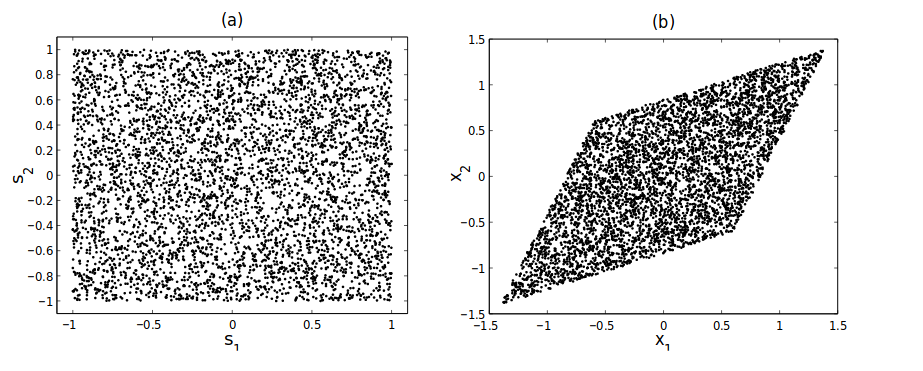
\includegraphics[scale=0.25]{linica.png}
	\end{center}
\end{frame}

\begin{frame}
\frametitle{قضیه‌ی 
\lr{Darmois-Skitovich}
}
اگر متغیر‌های تصادفی غیرگوسی باشند، مخلوط‌های خطی آن‌ها جدایی‌پذیر هستند.
\footnotesize{[\lr{Darmois-Skitovich∼1950}]}
\begin{theorem}
	\label{darmois_skitovic}
	فرض کنید 
	$X_1,X_2, \dots, X_n$
	متغیرهای تصادفی مستقل باشند. متغیر‌های تصادفی 
	$Y_1,Y_2$
	ر ا به شکل زیر تعریف کنید:
	\begin{equation}
	\begin{cases}
	Y_1 = a_1X_1 + a_2 X_2 + \dots a_NX_N\\
	Y_2 = b_1X_1 + b_2 X_2 + \dots b_NX_N
	\end{cases}
	\end{equation}
	اگر 
	$Y_1$
	و 
	$Y_2$
	مستقل باشند، تمام $X_k$ هایی که برای آن‌ها
	$a_kb_k \neq 0$
	است، گوسی هستند.
\end{theorem}
\end{frame}


\begin{frame}
\frametitle{نتایج پیشین: ترکیب‌های غیرخطی}
\begin{itemize}
	\item
	\textbf{	مسئله‌ی جداسازی کور مخلوط‌های غیرخطی:}

	\begin{figure}
		\centering
		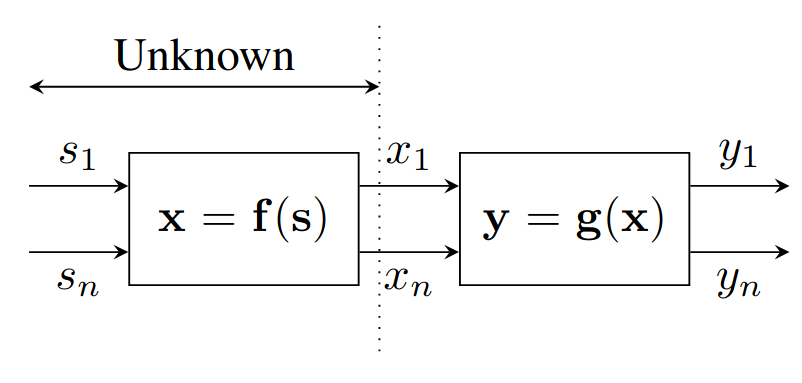
\includegraphics[scale=0.27]{BSS.png}
	\end{figure}
	
	\begin{itemize}
		\item 
		بردار منابع:
		$\mathbf{s} \in \mathbb{R}^n$
		\vspace{0.2cm}
		\item
	 بردار مشاهدات:		
	 	$\mathbf{x} \in \mathbb{R}^n$
	 	
	 	\vspace{0.2cm}
	 	\item
	 	
	 	تابع مخلوط‌کننده:
	 	$\mathbf{x} = \mathbf {f\big(s\big)}$
	 	\vspace{0.2cm}
	 	\item
	 	تابع جداسازی
	 	$\mathbf{s} = \mathbf {g\big(x\big)}$
	\end{itemize}
\end{itemize}
\end{frame}





\begin{frame}
\frametitle{جدایی‌پذیری مخلوط‌های غیرخطی}
{
	\setbeamercolor{block title}{use=example text,fg=white,bg=example text.fg!75!black}
	\setbeamercolor{block body}{parent=normal text,use=block title example,bg=block title example.bg!10!bg}
	\begin{block}{مخلوط‌های غیر خطی جدایی‌پذیر نیستند.}
		در ترکیب‌های غیرخطی متغیر‌های تصادفی، جداسازی غیرممکن است:
		\begin{equation*}
		\begin{cases}
		
		S_1 = \mathrm{Rayleigh}(\sigma)\\
		S_2 = \mathrm{Uniform} [0, 2\pi]
		\end{cases}
		\implies
		Y_1 = S_1 \cos (S_2) \perp \!\!\! \perp Y_2 =  S_1 \sin (S_2)
		\end{equation*}
	\end{block}
}
{
	\setbeamercolor{block title}{use=alerted text,fg=white,bg=alerted text.fg!75!black}
	\setbeamercolor{block body}{parent=normal text,use=block title alerted,bg=block title alerted.bg!10!bg}
	
	\pause
	\begin{block}{روابط زمانی کمک می‌کنند.}
		تابع فوق، استقلال فرآیند‌های تصادفی را حفظ نمی‌کند!
		\footnotesize{[\lr{Hosseini et al., 2003}]}
		
		\begin{align*}
		R_{y_1y_2}(t, t+1) &= \mathbb{E}\big[{y_1(t+1)y_2(t)}\big]\\
		&= \mathbb{E}\Big[s_1(t+1)s_1(t)\Big]
		\mathbb{E}\Big[\cos\big(s_2(t+1)\big)\sin\big(s_2(t)\big)\Big]
		\end{align*}
		
	\end{block}
}

\begin{block}	\label{thm1subgaussian}
	برای هر متغیّر تصادفی زیر--گاوسی 
	\lr{$X$}
	با متوسّط
	\lr{$\mu = \mathbb{E}[X]$}
	و پارامتر
	\lr{$\sigma$}
	داریم:
	\begin{equation}
	\mathbb{P}[|X-\mu|\geq t] \leq 2e^{-\frac{t^2}{2\sigma^2}}
	\end{equation}
\end{block}
\end{frame}


\begin{frame}
\frametitle{فرآیند‌های غیرایستان}
\begin{itemize}
	\item
	منابع غیر ایستان هستند.
	\begin{figure}
		\centering
		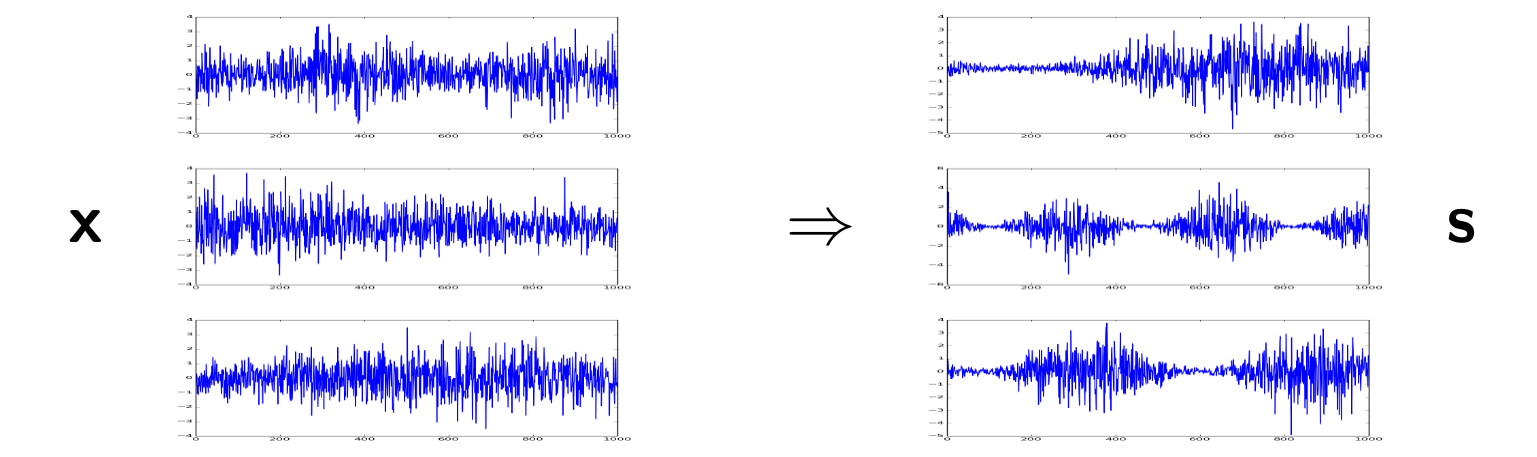
\includegraphics[scale=0.19]{nonstat.png}
	\end{figure}
	\item
	به عنوان مثال واریانس آن‌ها تغییر می‌کند:
	
	$$s_i(t) \sim \mathcal{N} \Big(0, \sigma_i (t)\Big)$$
	\item
	\textbf{جدایی‌پذیری:}
	\begin{itemize}
		\item
		مخلوط‌ خطی آن‌ها جدایی‌پذیر است.
		\footnotesize{\lr{[Pham and Cardoso, 2002]}}
		\item
		در مورد مخلوط‌های غیر خطی: 
		\textbf{قضیه نداریم}. \\
		\footnotesize{شبیه‌سازی‌ها امیدوار کننده هستند.}
		
	\end{itemize}
\end{itemize}
\end{frame}


\begin{frame}
\frametitle{
	ایده‌ی استفاده از مشتق}
\textbf{ایده:}
با وجود غیرخطی بودن تابع مخلوط کننده، مشتقات منابع به صورت موضعاً خطی مخلوط می‌شوند.
\footnotesize{\lr{[Ehsandoust et al. 2017]}}

\begin{equation*}
\frac{dx_i}{dt} = \sum_{j = 1}^{n} \frac{\partial f_i}{\partial s_j} \frac{ds_j}{dt}
\implies
\nabla\mathbf{x} = \mathbf{J}_{\mathbf{f}; t}(\mathbf{s})\nabla\mathbf{s}
\end{equation*}

\begin{figure}
	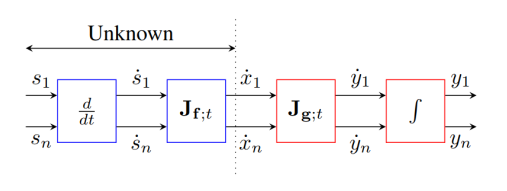
\includegraphics[scale=0.5]{Derv.png}
\end{figure}

\end{frame}

\begin{frame}
\frametitle{
	یادگیری بر مبنای تمایز زما‌ن‌ها
	(\lr{TCL})
}

این روش در سال ۲۰۱۶ در 
\footnotesize{\lr{[Hyvarinen and Morioka, 2016]}}
ارائه شد.
\begin{figure}
	\makebox[\textwidth][c]{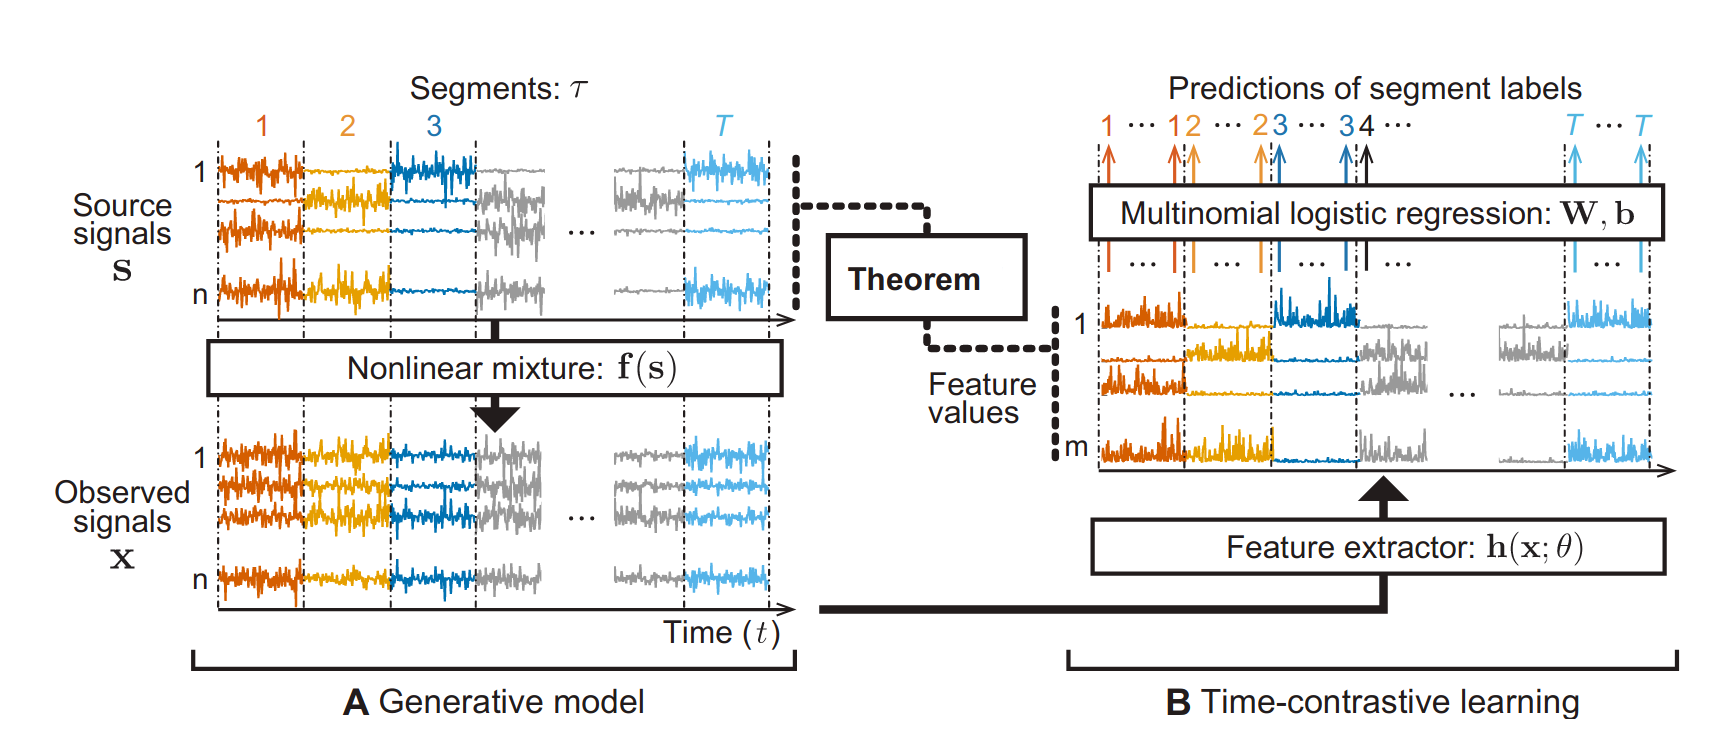
\includegraphics[width=1.2\textwidth]{TCL.png}}
\end{figure}
\end{frame}

\begin{frame}
\frametitle{
	\lr{TCL}
	منابع را جدا می‌کند!
}
{
	\setbeamercolor{block title}{use=alerted text,fg=white,bg=alerted text.fg!75!black}
	\setbeamercolor{block body}{parent=normal text,use=block title alerted,bg=block title alerted.bg!10!bg}
	\begin{theorem}
		فرض کنید توزیع منابع به صورت زیر باشد:
		\begin{equation*}
		\log p_\tau(s_i)=    \lambda_{i,1}(\tau) q(s_i) - \log Z( \lambda_{i,1}(\tau))
		\label{eq:p_tau_simple}
		\end{equation*}
		همچنین فرض کنید 
		فرض کنید ماتریس 
		$\mathbf{L}$
		با المان‌های 
		$$[\mathbf{L}]_{\tau, i} = 
		\lambda_{i, 1}(\tau) - \lambda_{i, 1}(1) \
		\;\;\;\;
		\tau = 1, \dots, T, \;\;
		i = 1, \dots, n
		$$
		داری رتبه‌ی ستونی کامل باشد. در حدی که بی‌‌شمار نمونه‌ی زمانی داریم و 
		\lr{TCL} 
		را اجرا کنیم،
		$\mathbf{A} \in \mathbb{R}^{n\times n}$
		و
		$\mathbf{d} \in \mathbb{R}^n$
		وجود دارند که:
		\begin{equation*}
		q(\mathbf{s}_t) = \mathbf{Ah}(\mathbf{x}_t, \theta) + \mathbf{d}
		\end{equation*}
	\end{theorem}
}
\end{frame}


\begin{frame}
\frametitle{
	\centering{یادگیری بر مبنای تمایز بین جایگشت‌ها}
(PCL)
}

\begin{columns}

\begin{column}{0.5\textwidth}
\begin{figure}
	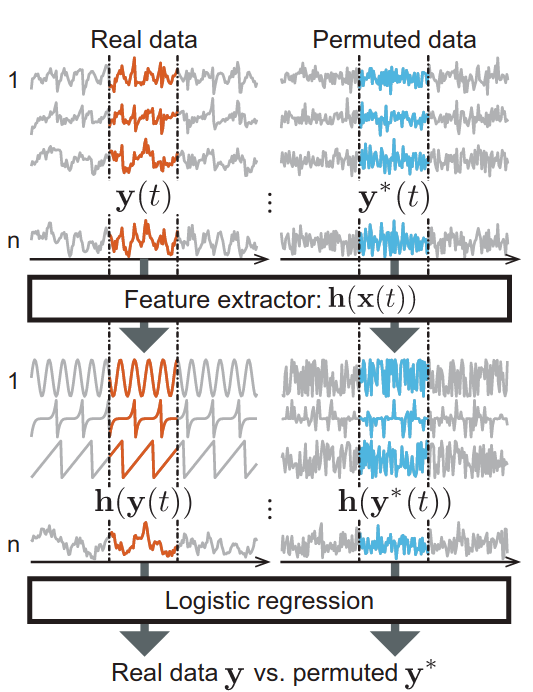
\includegraphics[scale=0.3]{PCL_over.png}
\end{figure}
\end{column}

\begin{column}{0.5\textwidth}
\lr{Original Data:}
$$\mathbf{y}(t) = \Big(\mathbf{x}(t), \mathbf{x}(t-1)\Big)$$

\lr{Permuted Data:}
$$\mathbf{y}^*(t) = \Big(\mathbf{x}(t), \mathbf{x}(t^*)\Big)$$
\end{column}
\end{columns}
\end{frame}

\begin{frame}
\frametitle{
یادگیری بر مبنای تمایز بین جایگشت‌ها
(PCL)
}

{
	\setbeamercolor{block title}{use=alerted text,fg=white,bg=alerted text.fg!75!black}
	\setbeamercolor{block body}{parent=normal text,use=block title alerted,bg=block title alerted.bg!10!bg}
\begin{theorem}
فرض‌ کنید داده‌ها از مدل غیرخطی 
$\mathbf{x}(t) = \mathbf{f}(\mathbf{s}(t_))$
پیروی کنند. اگر
\vspace{0.4cm}

1)
$\mathbf{f}: \mathbb{R}^n \to \mathbb{R}^n$
تابعی وارون‌پذیر و هموار باشد.
\vspace{0.4cm}

2)
منابع 
$s_i(t)$
ایستان بوده و مستقل باشند.
\vspace{0.4cm}

3)
$(s_i(t), s_i(t-1))$
شبه-گوسی نبوده و به صورت یکنواخت وابسته باشند.
(شرایطی قوی‌تر از رابطه‌ی زمانی و غیرگوسی بودن)
\vspace{0.4cm}

با اعمال 
\lr{TCL}
با 
$\mathbf{dim}(h)  =\mathbf{dim}(x) $
داریم:

$$s_i(t) = k_i(h_j(\mathbf{x}(t)))$$


\end{theorem}
}

\end{frame}


\begin{frame}
\frametitle{الگوریتم جداسازی}
ایده از «گرادیان تصادفی» اطلاعات متقابل در
\lr{\scriptsize{[Babaie-Zadeh, 2002]}}

\begin{figure}[h!]
	\centering
	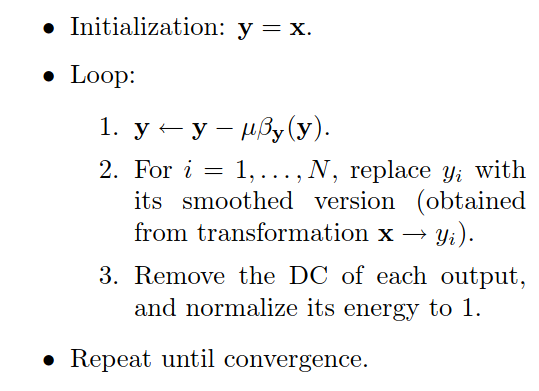
\includegraphics[width=0.5\textwidth]{./Figures/alg.png}
	\hfill
	
\includegraphics[width=0.5\textwidth]{./Figures/snr.png}
\end{figure}
\end{frame}


\begin{frame}
\frametitle{
	ادامه‌ی کار در پروژه‌ی کارشناسی ۲}

{
	\setbeamercolor{block title}{use=alerted text,fg=white,bg=alerted text.fg!75!black}
	\setbeamercolor{block body}{parent=normal text,use=block title alerted,bg=block title alerted.bg!10!bg}
	\begin{block}{هدف غایی}
		تعمیم 
		یک نظریه‌ی وجدت‌ یافته برای جداسازی غیرخظی منابع با روابط زمانی؟ 
		
		فهم دقیق‌تر محدودیت‌های روش‌های موجود
	\end{block} 
}

{
	\setbeamercolor{block title}{use=example text,fg=white,bg=example text.fg!75!black}
	\setbeamercolor{block body}{parent=normal text,use=block title example,bg=block title example.bg!10!bg}
	\begin{block}{تعمیم 
			\lr{TCL}	
		}
		تعمیم قضیه‌ی جدایی پذیری 
		\lr{TCL}
		به منابع «غیرایستان شبه-نمایی»:
		\begin{equation*} 
		\log p_\tau(s_i)=  q_{i,0}(s_i) + \sum_{v=1}^V \lambda_{i,v}(\tau) q_{i,v}(s_i) - \log Z( \lambda_{i,1}(\tau),\ldots,\lambda_{i,v}(\tau))
		\label{eq:p_tau}
		\end{equation*}
	\end{block} 
}

	\begin{block}{الگوریتم مبتنی بر 
	\lr{HSIC}	
	}
	استفاده از معیار استقلال هیلبرت-اشمیت (HSIC) به جای اطلاعات متقابل برای طراحی الگوریتم جداسازی کور
	\end{block} 

\end{frame}



\begin{frame}
\frametitle{مراجع}
\footnotesize{
\begin{flushleft}
	
\begin{latin}
[1] M. Babaie-Zadeh, On Blind Source  Separation in Convolutive and
 Nonlinear Mixtures. Ph.D. Thesis, INPG and Sharif, 2002.
\vspace{0.5cm}

[2]  S. Harmeling, A. Ziehe, M. Kawanabe, and K.-R. Müller, “Kernel Based Nonlinear Blind Source Separation”, Neural Computation,
 vol.15, no.5, pp.1089–1124, 2003.
\vspace{0.5cm}


[3] A. Hyvarinen and H. Morioka, “Unsupervised Feature Extraction
by Time-Contrastive Learning and Nonlinear ICA”, NIPS, 2016.
\vspace{0.5cm}

[4] A. Hyvarinen and H. Morioka, “Nonlinear ICA of Temporally Dependent Stationary Sources”, AISTAT, 2017.
\vspace{0.5cm}


\end{latin}

\end{flushleft}
}
\end{frame}

\begin{frame}
\frametitle{مراجع}
\footnotesize{
	\begin{flushleft}
		
		\begin{latin}
			[5] B. Ehsandoust, M. Babaie-Zadeh, B. Rivet, and C. Jutten, “Blind
	Source Separation in Nonlinear Mixtures: Separability and a Basic Algorithm”, IEEE Transactions on Signal Processing, 2017.
			\vspace{0.5cm}
			
			
			[6] S. Hosseini and C. Jutten, “On the separability of nonlinear mixtures of temporally correlated sources”, IEEE Signal Processing
 	Letters,  2003.
			\vspace{0.5cm}
			
			[7] X. Zhang, L. Song, A. Gretton, and A. J. Smola, “Kernel Measures
 of Independence for non-iid Data”, NIPS, 2009.
			
			
			
		\end{latin}
	
\end{flushleft}
}
\end{frame}




\end{document}